% Created 2015-06-03 Wed 16:31
\documentclass[11pt]{article}
\usepackage[utf8]{inputenc}
\usepackage[T1]{fontenc}
\usepackage{graphicx}
\usepackage{longtable}
\usepackage{float}
\usepackage{wrapfig}
\usepackage{soul}
\usepackage{amssymb}
\usepackage{hyperref}
\usepackage{geometry}
\usepackage{tikz}

\title{notes}
\author{Eike Ritter}
\date{03 June 2015}

\begin{document}

\maketitle

\setcounter{tocdepth}{3}
\tableofcontents
\vspace*{1cm}

\section{Stateful injective agreement}
\label{sec-1}


\begin{enumerate}
\item Prove non-injective correspondence between $begin(e1(M_1))$ and
   $end(e2(M_2))$ as usual, it works! The use of sequence predicate
   chains correctly the two sessions, since the state produced by the
   begin event needs to be reachable in order for the end event to
   succeed.
\item Once non-injectivity is proven, treat $e2(M_2)$ both as a begin
   (now called end1) and as an end (called end2) event, inserting the
   clauses:
   \begin{align*}
     H \wedge end1(e2(M_2)) \Rightarrow mid  \\
     H \wedge mid \Rightarrow end2(e2(M_2))
   \end{align*}
   Intuitively this forces the resolution to produce clauses that
   contain $end1$ on the l.h.s. and $end2$ on the r.h.s.
\item Saturate the clauses, ensuring that Horn clauses of the form $H
   \wedge end1(e2(M_2)) \Rightarrow C$ are not eliminated as redundant
   because $H \Rightarrow C$ is present. It is important to note that
   this change in saturation does not influence termination, rather it
   \emph{doubles} the amount of clauses produced in case both $H \wedge
   end1(e1(M_2)) \Rightarrow C$ and $H \Rightarrow C$ are present.
\item Look for rules in the saturation of the form:
   $$  H \wedge end1(e2(M_2)) \Rightarrow end2(e2(M'_2)) $$
   \emph{Conjecture:}
   Let $\sigma=mgu(M_2, M'_2)$. If two occurrences of $begin(e1(M_1))$
   are forced to unify in $H$ then the protocol is secure, otherwise a
   potential attack is found. The intuitive reason why this should
   work is that if only one \emph{begin} event is found, and both \emph{end1}
   and \emph{end2} events appear in the clause, then in the abstraction one
   begin event could have generated two end events, hence there is a
   potential attack. If two begin events are present in the
   hypothesis, then they are marked with different terms, representing
   potentially different sessions of the process that executed the
   begin event. If unifying the \emph{end1} and \emph{end2} events triggers also
   the unification of the two instances of \emph{begin}, this means that
   the two occurrences represent one single session, hence the clause
   does not represent an attack.

   \textbf{This doesn't hold} as we were able to prove a counter example
   (protocol in test.pv that does not have injective agreement
   property).
\end{enumerate}
\section{Example:}
\label{sec-2}


   GateCard.pv generates the following clauses, when testing
   non-injective agreement between $permit(x,y) \Rightarrow add(x)$:
   \begin{flalign*}
   & s_1 \neq 0 \wedge att((s_1,0),y) \wedge seq(s,(s_1,0)) \Rightarrow end(permit(s_1,y)) & \\
   & s_1 \neq 0 \wedge att((s_1,0),y) \wedge seq(s,(s_1,0)) \Rightarrow seq((s_1,0),(0,0)) \\
   & s_1 \neq 0 \wedge seq((s_1,0),(0,0)) \wedge att((s_1,0),y) \wedge seq(s,(s_1,0)) \Rightarrow att((0,0),sign((s_1,y),K[])) \\
   & s_2 \neq 0 \wedge att((s_1,s_2),y) \wedge seq(s,(s_1,s_2)) \Rightarrow end(permit(s_2,y)) \\
   & s_2 \neq 0 \wedge att((s_1,s_2),y) \wedge seq(s,(s_1,s_2)) \Rightarrow seq((s_1,s_2),(s_1,0)) \\
   & s_2 \neq 0 \wedge seq((s_1,s_2),(s_1,0)) \wedge att((s_1,s_2),y) \wedge seq(s,(s_1,s_2)) \Rightarrow att((s_1,0),sign((s_2,y),K[])) \\
   & seq(s,s') \Rightarrow att(s',m[i]) \\
   & begin(add(m[i])) \wedge att((0,s_2),sign(m[i],L[])) \wedge seq(s,(0,s_2)) \Rightarrow seq((0,s_2),(m[i],0)) \\
   & s_1 \neq 0 \wedge begin(add(m[i])) \wedge att((s_1,0),sign(m[i],L[])) \wedge seq(s,(s_1,0)) \Rightarrow seq((s_1,0),(s_1,m[i]))
   \end{flalign*}
   When testing injective agreement we produce the following clauses:
   \begin{flalign*}
   & s_1 \neq 0 \wedge att((s_1,0),y) \wedge seq(s,(s_1,0)) \wedge mid \Rightarrow end2(permit(s_1,y)) & \\
   & s_1 \neq 0 \wedge att((s_1,0),y) \wedge seq(s,(s_1,0)) \wedge end1(permit(s_1,y)) \Rightarrow mid  \\
   & s_1 \neq 0 \wedge att((s_1,0),y) \wedge seq(s,(s_1,0)) \wedge end1(permit(s_1,y)) \wedge mid \Rightarrow seq((s_1,0),(0,0)) \\
   & s_1 \neq 0 \wedge seq((s_1,0),(0,0)) \wedge att((s_1,0),y) \wedge seq(s,(s_1,0)) \wedge end1(permit(s_1,y)) \wedge mid \\
   & \hspace{3em} \Rightarrow att((0,0),sign((s_1,y),K[])) \\
   & s_2 \neq 0 \wedge att((s_1,s_2),y) \wedge seq(s,(s_1,s_2)) \wedge mid \Rightarrow end2(permit(s_2,y)) \\
   & s_2 \neq 0 \wedge att((s_1,s_2),y) \wedge seq(s,(s_1,s_2)) \wedge end1(permit(s_2,y)) \Rightarrow mid \\
   & s_2 \neq 0 \wedge att((s_1,s_2),y) \wedge seq(s,(s_1,s_2)) \wedge end1(permit(s_2,y)) \wedge mid \Rightarrow seq((s_1,s_2),(s_1,0)) \\
   & s_2 \neq 0 \wedge seq((s_1,s_2),(s_1,0)) \wedge att((s_1,s_2),y) \wedge seq(s,(s_1,s_2)) \wedge end1(permit(s_2,y)) \wedge mid \\
   & \hspace{3em} \Rightarrow att((s_1,0),sign((s_2,y),K[])) \\
   & seq(s,s') \Rightarrow att(s',m[i]) \\
   & begin(add(m[i])) \wedge att((0,s_2),sign(m[i],L[])) \wedge seq(s,(0,s_2)) \Rightarrow seq((0,s_2),(m[i],0)) \\
   & s_1 \neq 0 \wedge begin(add(m[i])) \wedge att((s_1,0),sign(m[i],L[])) \wedge seq(s,(s_1,0)) \Rightarrow seq((s_1,0),(s_1,m[i]))
   \end{flalign*}
   Somehow we must record that the $m[i]$ generated by the card when
   adding a new token are \emph{fresh}, hence different from any other
   token produced.

   Saturation should produce the clause:
   $$ begin(add(m[i])) \wedge end1(permit(m[i],n[j])) \wedge begin(add(m[i'])) \Rightarrow end2(permit(m[i'],n[j'])) $$
   with the unification resulting in the following substitution:
   $$ \sigma = \{{i}/{i'}, {j}/{j'}\} $$

\section{Learned lesson:}
\label{sec-3}

\begin{enumerate}
\item The simple idea of checking $end1 \implies end2$ is sound but
      could give rise to false attacks. Instead of the \emph{mid} predicate
      we should use correctly the \emph{seq} predicate to capture the state
      dependency between \emph{end1} and \emph{end2}. As a solution for reaching
      $end1 \implies end2$ in stateless protocols it is possible to
      insert a dummy $seq(\phi, \phi)$ predicate so that the rules for
      \emph{end1} and \emph{end2} can be chained.
\item Using the \emph{seq} predicate instead of \emph{mid} is not good for
      non-termination.
\item What is not captured is the information on the state
      $$ (0,0) \to (m[i],0) \to (0,0) \to (m[j],0) $$
      it works because we know by freshness that $i \neq j$, hence we 
      cannot reach the state $end1(x) \implies end2(x)$, because it would
      force unification of i and j.
\item Idea:
\end{enumerate}
   
\begin{enumerate}
\item the attacker knowledge does not increase in the second
         round of the protocol
\item the control flow in the second iteration is the same as in
         the first iteration, so it makes no sense to go on in this
         cycle.
\end{enumerate}
\section{Problems with Locks}
\label{sec-4}

\subsection{Visible intermediate states}
\label{sec-4.1}

\begin{enumerate}
\item Locks are too coarse. For example the process:
      \[lock(s_1,s_2,s_3); new\ a; out(a); set\ a \in s_1; set\ a \in s_2;\]
      would generate:
      \[att(a[0,0,x3])\]
      \[implies(a[0,0,x3], a[1,0,x3])\]
      \[implies(a[1,0,x3], a[1,1,x3])\]
      and hence the predicate
      \[att(a[1,0,x3])\]
      is reachable, although one would like only the final state, namely
      \[att(a[1,1,x3])\]
      to be visible from the outside.
\end{enumerate}
\subsection{Set-abstraction multi-value interleavings}
\label{sec-4.2}

\begin{enumerate}
\item For the set abstraction, one of the problems is the locality of the states in transitions
      \[att(sign(xm[x1,x2,x3],xc[1],k[])) \implies implies(xm[x1,x2,x3],xm[x1,1,x3])\]
      \[att(sign(xm[x1,x2,x3],xc[1],k[])) \implies implies(xc[1],xc[2])\]
\item we get all the diamond of interleavings:

      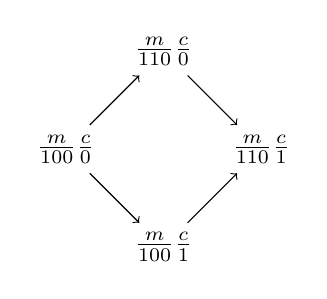
\begin{tikzpicture}[node distance=5em]
      \node (a) {${{m}\over{100}}{{c}\over{0}}$};
      \node [above right of=a] (b) {${{m}\over{110}}{{c}\over{0}}$};
      \node [below right of=a] (c) {${{m}\over{100}}{{c}\over{1}}$};
      \node [below right of=b] (d) {${{m}\over{110}}{{c}\over{1}}$};
      \draw [->] (a) to (b);
      \draw [->] (b) to (d);
      \draw [->] (a) to (c);
      \draw [->] (c) to (d);
      \end{tikzpicture}
\item which is bad because the intermediate states should not be visible. We would like to see the following state transition system:

      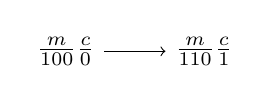
\begin{tikzpicture}[node distance=5em]
      \node (a) {${m \over 100}{c \over 0}$};
      \node [right of=a] (b) {${m \over 110}{c \over 1}$};
      \draw [->] (a) to (b);
      \end{tikzpicture}
\item we could solve it by:
      $$ att(sign(xm[x1,x2,x3],xc[1],k[])) \implies implies([xm[x1,x2,x3],xc[1]],[xm[x1,1,x3],xc[2]]) $$
      $$ att(sign(m[x1,x2,x3],xc[1],k[])) \wedge &implies([xm[x1,x2,x3],xc[1]],[xm[x1,1,x3],xc[2]])
      \implies att(sign(m[x1,1,x3],xc[2],k[]))\] $$
\end{enumerate}
$^{1}$ FOOTNOTE DEFINITION NOT FOUND: 0

$^{2}$ FOOTNOTE DEFINITION NOT FOUND: 1


\end{document}
